\section{Examples and the list}\label{sec:examples}
\providecommand{\NList}{}\renewcommand{\NList}{375}
\providecommand{\NPfail}{}\renewcommand{\NPfail}{11}
\providecommand{\NScope}{}\renewcommand{\NScope}{364}
\providecommand{\NBdryEnum}{}\renewcommand{\NBdryEnum}{327}
\providecommand{\NBdryIP}{}\renewcommand{\NBdryIP}{37}
\providecommand{\NMinNegZero}{}\renewcommand{\NMinNegZero}{195}
\providecommand{\NMinNegPos}{}\renewcommand{\NMinNegPos}{169}
\providecommand{\NMinNegTwo}{}\renewcommand{\NMinNegTwo}{57}
\providecommand{\NMinNegFour}{}\renewcommand{\NMinNegFour}{89}
\providecommand{\NMinNegSix}{}\renewcommand{\NMinNegSix}{21}
\providecommand{\NMinNegEight}{}\renewcommand{\NMinNegEight}{2}
\providecommand{\NBelts}{}\renewcommand{\NBelts}{179}
\providecommand{\NRealised}{}\renewcommand{\NRealised}{340}
\providecommand{\NRemaining}{}\renewcommand{\NRemaining}{24}
\providecommand{\NCorankOne}{}\renewcommand{\NCorankOne}{16}
\providecommand{\NCorankMax}{}\renewcommand{\NCorankMax}{4}
\providecommand{\NFailSheet}{}\renewcommand{\NFailSheet}{10}
\providecommand{\NFailFill}{}\renewcommand{\NFailFill}{24}
\providecommand{\NFailLocal}{}\renewcommand{\NFailLocal}{18}
\providecommand{\NVertexSets}{}\renewcommand{\NVertexSets}{668}
\providecommand{\NAdmSets}{}\renewcommand{\NAdmSets}{613}
\providecommand{\NAdm}{}\renewcommand{\NAdm}{612}
\providecommand{\NHexFree}{}\renewcommand{\NHexFree}{470}
\providecommand{\NHexFreeSmooth}{}\renewcommand{\NHexFreeSmooth}{8}
\providecommand{\NHexSets}{}\renewcommand{\NHexSets}{143}
\providecommand{\NHex}{}\renewcommand{\NHex}{142}
\providecommand{\NHexProj}{}\renewcommand{\NHexProj}{83}
\providecommand{\NHexNoProj}{}\renewcommand{\NHexNoProj}{59}
\providecommand{\NHexAone}{}\renewcommand{\NHexAone}{20}
\providecommand{\NHexAtwo}{}\renewcommand{\NHexAtwo}{55}
\providecommand{\NHexMixed}{}\renewcommand{\NHexMixed}{18}
\providecommand{\NCorBHexFree}{}\renewcommand{\NCorBHexFree}{118}
\providecommand{\NHexOne}{}\renewcommand{\NHexOne}{29}
\providecommand{\NCorBHexOne}{}\renewcommand{\NCorBHexOne}{10}
\providecommand{\NHexMany}{}\renewcommand{\NHexMany}{54}
\providecommand{\NCorBHexMany}{}\renewcommand{\NCorBHexMany}{33}
\providecommand{\NCorBHex}{}\renewcommand{\NCorBHex}{43}
\providecommand{\NScopeAll}{}\renewcommand{\NScopeAll}{447}
\providecommand{\NCorBAll}{}\renewcommand{\NCorBAll}{161}
\providecommand{\NCorBAoneWit}{}\renewcommand{\NCorBAoneWit}{18}
\providecommand{\NCorBAtwoWit}{}\renewcommand{\NCorBAtwoWit}{22}
\providecommand{\NCorBMixedWit}{}\renewcommand{\NCorBMixedWit}{10}
\providecommand{\NThmCBases}{}\renewcommand{\NThmCBases}{367}
\providecommand{\NThmCGlobal}{}\renewcommand{\NThmCGlobal}{191}
\providecommand{\NThmCHexBases}{}\renewcommand{\NThmCHexBases}{72}
\providecommand{\NHexRealAone}{}\renewcommand{\NHexRealAone}{19}
\providecommand{\NHexRealAtwo}{}\renewcommand{\NHexRealAtwo}{66}
\providecommand{\NHexProfAtwo}{}\renewcommand{\NHexProfAtwo}{71}
\providecommand{\NHexFreeKzero}{}\renewcommand{\NHexFreeKzero}{87}
\providecommand{\NCorBFail}{}\renewcommand{\NCorBFail}{286}
\providecommand{\NBeltsStrict}{}\renewcommand{\NBeltsStrict}{171}
\providecommand{\NBeltsCrossPoly}{}\renewcommand{\NBeltsCrossPoly}{8}
\providecommand{\NBeltsChecked}{}\renewcommand{\NBeltsChecked}{3{,}389}
\providecommand{\NBeltsCross}{}\renewcommand{\NBeltsCross}{28}


This section makes the objects of the paper explicit on five hypersurfaces and reports what the computations on the
list of admissible polytopes show. Section~\ref{ssec:x9} treats $X_9$ by hand: it has four nodes and $\operatorname{rank}K=1$,
and a single disc through the four nodes realises the generator of $K$ as a tropical $2$-cycle, so that
Theorems~\ref{thm:main}--\ref{thm:res} and Corollary~\ref{cor:smooth} can be followed through one picture.
Section~\ref{ssec:x19x20} lists explicit generators of $K$ on $X_{19}$ and $X_{20}$; on $X_{20}$ two nodes are forced to
vanish on $K$, and Corollary~\ref{cor:smooth} then says that no relation among the vanishing spheres has all coefficients
nonzero. Section~\ref{ssec:hexexamples} gives one example on each branch of the $dP_6$ hexagon.
Section~\ref{ssec:list} describes the list, counts the polytopes to which the theorems apply and those on which the
equivalent conditions of Corollary~\ref{cor:smooth} hold, and records a computational verification of
Theorem~\ref{thm:real} on the bases of $435$ polytopes of the list, $\NScope$ without and $\NHexProfAtwo$ with
hexagonal two-faces. Section~\ref{ssec:evidence} collects the evidence for Conjecture~\ref{conj:strict}.

Throughout, the lattice points of $\Delta$ that are rays of $\Sigma'$ are numbered $n_0,n_1,\dots$ as in
Appendix~\ref{app:data}, a node parallelogram is written $q=(a,b,c,d)$ with $n_a+n_c=n_b+n_d$ and chosen diagonal
$\{a,c\}$ (through the centre at a pentagon or hexagon), and $e_i$ stands for the basis vector $e_{n_i}$ of $\Z^R$, so
that $\circv_q=e_b+e_d-e_a-e_c$. Vectors of $\Z^Q$ are written as combinations of the nodes: $q_1-q_2$ is the vector with
coordinate $1$ at $q_1$, $-1$ at $q_2$ and $0$ elsewhere.

\subsection{The example \texorpdfstring{$X_9$}{X9}}\label{ssec:x9}
The polytope $\Delta_9$ of \cite{Paper5} has nine vertices, listed in Appendix~\ref{app:data-x9}, one $dP_7$ pentagon
with vertices $n_3,n_4,n_5,n_6,n_8$ and centre $n_{10}=(-2,-1,0,0)$, and two unit squares
$\{n_2,n_6,n_3,n_7\}$ and $\{n_2,n_5,n_4,n_7\}$; its other two-faces are unimodular triangles. It is admissible, it
satisfies~\ref{hyp:P} with the fan $\Sigma'$ of Appendix~\ref{app:data-x9}, and by Theorem~\ref{thm:U} it has a base
$B=B'_\sigma$. So Theorems~\ref{thm:main}--\ref{thm:res} apply to it.

\emph{The nodes and $K$.} The pentagon contributes two node parallelograms and each square one:
\[
q_1=(n_3,n_6,n_{10},n_8),\quad q_2=(n_2,n_6,n_3,n_7),\quad q_3=(n_4,n_5,n_{10},n_8),\quad q_4=(n_2,n_5,n_4,n_7),
\]
with $q_1,q_3$ in the pentagon. Their circuits are
\[
\begin{aligned}
\circv_{q_1}&=e_6+e_8-e_3-e_{10}, &\qquad \circv_{q_2}&=e_6+e_7-e_2-e_3,\\
\circv_{q_3}&=e_5+e_8-e_4-e_{10}, & \circv_{q_4}&=e_5+e_7-e_2-e_4.
\end{aligned}
\]
If $\sum_k\lambda_k\circv_{q_k}=0$, the coefficients of $e_{10}$, $e_6$ and $e_7$ give $\lambda_3=-\lambda_1$,
$\lambda_2=-\lambda_1$ and $\lambda_4=-\lambda_2$; conversely $\circv_{q_1}-\circv_{q_2}-\circv_{q_3}+\circv_{q_4}=0$. Hence
\[
K=\Z\,(q_1-q_2-q_3+q_4),
\]
and the relative Picard number of $\widehat X_9\to X'_9$ is $|Q|-\operatorname{rank}K=3$. The relation
$\lambda_{q_1}+\lambda_{q_3}=0$ holds because the centre $n_{10}$ occurs only in the circuits of the two pentagon nodes;
this is the tie of Remark~\ref{rem:tie}.

\emph{A cycle of node parallelograms.} Put $d_0=(4,2,1,1)$. Every node parallelogram has a pair of opposite sides
parallel to $d_0$:
\[
n_3-n_6=n_8-n_{10}=n_4-n_5=n_7-n_2=d_0 .
\]
Write $\varepsilon_1=[n_6,n_3]$, $\varepsilon_2=[n_{10},n_8]$, $\varepsilon_3=[n_5,n_4]$ and $\varepsilon_4=[n_2,n_7]$. Then $q_1$ has the sides
$\varepsilon_1,\varepsilon_2$, $q_3$ the sides $\varepsilon_2,\varepsilon_3$, $q_4$ the sides $\varepsilon_3,\varepsilon_4$ and $q_2$ the sides
$\varepsilon_4,\varepsilon_1$. So the four segments close up into a cycle $\varepsilon_1,\varepsilon_2,\varepsilon_3,\varepsilon_4$ in which consecutive
segments are opposite sides of one node parallelogram. The boundary of the disc constructed below runs through the
four nodes in this order.

\emph{Belt cycles.} The disc belongs to the simplest class of tropical $2$-cycles.

\begin{definition}[belt cycles]\label{def:belt}
A \emph{belt cycle} on $B$ is a tropical $2$-cycle $(S,j,v)$ in the sense of \cite[Def.~7.2]{CBM} such that $S$ is a disc
with one sheet and no interior edges or vertices, $S$ does not cross $\Gamma$, and $\partial S$ is a closed path in
$\Gamma$ along legs with vanishing vector $\pm v$ which passes every node it meets along two opposite legs and meets no
negative vertex.
\end{definition}

The field of a belt cycle is constant, since $S$ is a disc on which it is parallel; as a relative tropical
$2$-cycle (Section~\ref{ssec:cbm}) a belt cycle is the chain $v[S]$, with boundary network $v[\partial S]$, and its node
coefficients are supported on the nodes of $\partial S$.

\emph{The facet.} Let $\mathcal T$ be the unimodular triangulation of $\partial\Delta_9^\circ$ of the data accompanying the paper
(\coderepo; see Appendix~\ref{app:data}), and let $u_0=(0,1,-1,-1)$ and
\[
\begin{gathered}
u_1=(1,-1,-1,-1),\quad u_2=(0,0,1,-1),\quad u_3=(-1,2,1,-1),\\ u_4=(-1,2,0,0),\quad u_5=(-1,2,-1,1).
\end{gathered}
\]
In $\mathcal T$ the vertex $u_0$ is joined by edges to $u_1,\dots,u_5$, and $[u_0,u_i,u_{i+1}]$ is a triangle of $\mathcal T$
for $i=1,\dots,5$ (indices modulo $5$). Recall from Section~\ref{ssec:gross} that the facets $F_u$ of
$\nabla^{\check h}$ correspond to the lattice points $u$ of $\partial\Delta^\circ$ and its two-faces $F_{uu'}=F_u\cap F_{u'}$
to the edges of $\mathcal T$, and that $\Gamma$ lies in the union of the two-faces and meets no facet interior. All six
vectors $u_i$ annihilate $d_0$. So the five two-faces $F_{u_0u_i}$ of the facet $F_{u_0}$, and the five edges
$F_{u_0}\cap F_{u_i}\cap F_{u_{i+1}}$, contain the direction $d_0$. For an edge $[u,u']$ of $\mathcal T$ and an edge
$[n,n']$ of $\Sigma'$ we write $([u,u'],[n,n'])$ for the arc of $\Gamma$ in $F_{uu'}$ whose legs have lower support
$\{n,n'\}$ (Proposition~\ref{prop:L2}(2)); its legs have vanishing vector $\pm(n'-n)$ and covector $\pm(u'-u)$
(Lemma~\ref{lem:monodromy}).

\emph{The closed path.} Let $\partial S\subset\Gamma$ be the following union of arcs:
\begin{itemize}
\item from $p_{q_1}$ along $([u_0,u_1],\varepsilon_1)$ and $([u_0,u_5],\varepsilon_1)$ to $p_{q_2}$;
\item from $p_{q_2}$ along $([u_0,u_5],\varepsilon_4)$, $([u_0,u_4],\varepsilon_4)$ and $([u_0,u_3],\varepsilon_4)$ to $p_{q_4}$;
\item from $p_{q_4}$ along $([u_0,u_3],\varepsilon_3)$, $([u_0,u_2],\varepsilon_3)$ and $([u_0,u_1],\varepsilon_3)$ to $p_{q_3}$;
\item from $p_{q_3}$ along $([u_0,u_1],\varepsilon_2)$ back to $p_{q_1}$.
\end{itemize}
Consecutive arcs with the same lower support meet at the positive vertices $([u_0,u_i,u_{i+1}],\sigma)$, one on each of
the five edges $F_{u_0}\cap F_{u_i}\cap F_{u_{i+1}}$, and the nodes are $p_{q_1}=([u_0,u_1],q_1)$,
$p_{q_3}=([u_0,u_1],q_3)$, $p_{q_4}=([u_0,u_3],q_4)$ and $p_{q_2}=([u_0,u_5],q_2)$. In all, $\partial S$ consists of $18$
legs; it passes through the four nodes and five positive vertices and meets no negative vertex. At each node it follows
two opposite legs, those over $\varepsilon_1,\varepsilon_2$ at $q_1$, over $\varepsilon_2,\varepsilon_3$ at $q_3$, over $\varepsilon_3,\varepsilon_4$ at $q_4$
and over $\varepsilon_4,\varepsilon_1$ at $q_2$. Figure~\ref{fig:x9} shows the configuration.

\begin{figure}[ht]
\centering
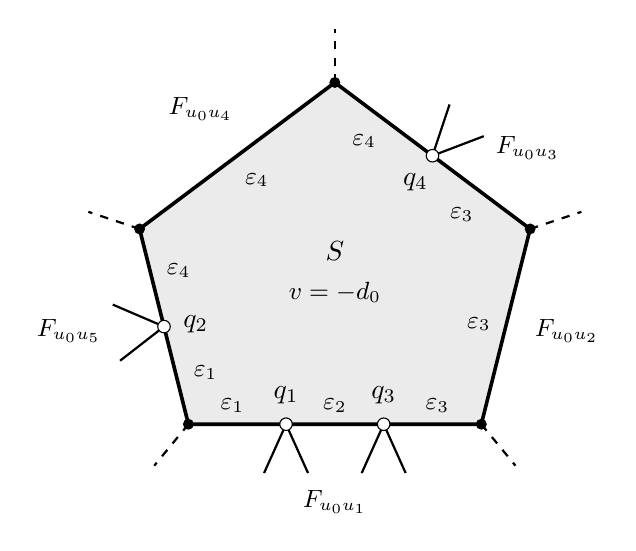
\begin{tikzpicture}[scale=0.62,
  leg/.style={line width=1.3pt},
  stub/.style={line width=0.8pt},
  nodev/.style={circle,draw,fill=white,inner sep=1.6pt},
  posv/.style={circle,fill=black,inner sep=1.4pt}]
  \fill[black!8] (0,4)--(4,1)--(3,-3)--(-3,-3)--(-4,1)--cycle;
  \draw[leg] (0,4)--(4,1)--(3,-3)--(-3,-3)--(-4,1)--cycle;
  \draw[stub,dashed] (0,4)--(0,5.1);
  \draw[stub,dashed] (4,1)--(5.05,1.35);
  \draw[stub,dashed] (3,-3)--(3.7,-3.85);
  \draw[stub,dashed] (-3,-3)--(-3.7,-3.85);
  \draw[stub,dashed] (-4,1)--(-5.05,1.35);
  \draw[stub] (-1,-3)--(-1.45,-4.0); \draw[stub] (-1,-3)--(-0.55,-4.0);
  \draw[stub] (1,-3)--(0.55,-4.0);   \draw[stub] (1,-3)--(1.45,-4.0);
  \draw[stub] (-3.5,-1)--(-4.55,-0.55); \draw[stub] (-3.5,-1)--(-4.4,-1.7);
  \draw[stub] (2,2.5)--(2.35,3.55); \draw[stub] (2,2.5)--(3.05,2.9);
  \foreach \p in {(0,4),(4,1),(3,-3),(-3,-3),(-4,1)} \node[posv] at \p {};
  \node[nodev] at (-1,-3) {}; \node[nodev] at (1,-3) {};
  \node[nodev] at (-3.5,-1) {}; \node[nodev] at (2,2.5) {};
  \node at (-1,-2.4) {$q_1$}; \node at (1,-2.4) {$q_3$};
  \node at (-2.85,-0.95) {$q_2$}; \node at (1.65,1.95) {$q_4$};
  \node at (-2.1,-2.62) {\small$\varepsilon_1$}; \node at (0,-2.62) {\small$\varepsilon_2$}; \node at (2.1,-2.62) {\small$\varepsilon_3$};
  \node at (-2.65,-1.95) {\small$\varepsilon_1$}; \node at (-3.2,0.15) {\small$\varepsilon_4$};
  \node at (-1.6,2.0) {\small$\varepsilon_4$}; \node at (0.6,2.8) {\small$\varepsilon_4$};
  \node at (2.6,1.3) {\small$\varepsilon_3$}; \node at (2.95,-0.95) {\small$\varepsilon_3$};
  \node at (0,-4.6) {\small$F_{u_0u_1}$};
  \node at (4.75,-1.1) {\small$F_{u_0u_2}$};
  \node at (3.95,2.65) {\small$F_{u_0u_3}$};
  \node at (-2.75,3.45) {\small$F_{u_0u_4}$};
  \node at (-5.45,-1.1) {\small$F_{u_0u_5}$};
  \node at (0,0.55) {$S$}; \node at (0,-0.3) {\small$v=-d_0$};
\end{tikzpicture}
\caption{The belt cycle of $X_9$, schematically: the boundary of the facet $F_{u_0}$ seen along $d_0$. The five two-faces
$F_{u_0u_i}$ met by $\partial S$ appear as sides and the five positive vertices of $\partial S$ as corners ($\bullet$); the
four nodes are the circles. Thick lines are the $18$ legs of $\partial S$, labelled by their lower supports
$\varepsilon_1,\dots,\varepsilon_4$; the two other legs at each node and the third leg at each positive vertex (dashed) leave
$F_{u_0}$ and are drawn as stubs. The disc $S$ (shaded) spans $\partial S$ inside $F_{u_0}$, with the constant field
$-d_0$.}\label{fig:x9}
\end{figure}

\emph{The disc.} Let $S$ be the disc bounded by $\partial S$ formed by the $26$ triangles $(b_e,b_f,b_C)$ of the
barycentric subdivision $\mathfrak K_0$ of $\mathscr P$ listed in the accompanying data (\coderepo). Its triangles lie in three maximal
cells of $\mathscr P$, all with facet index $u_0$, and $S$ meets the two-faces of $\nabla^{\check h}$ only along
$\partial S$. Orient $S$ so that $\partial S$ passes through the nodes in the order $q_1,q_2,q_4,q_3$, and give it the
constant field $v=-d_0$.

\begin{lemma}\label{lem:x9belt}
$(S,j,v)$ is a belt cycle, and $\rho(S)=q_1-q_2-q_3+q_4$. In particular $\rho(S)$ generates $K$.
\end{lemma}

\begin{proof}
We check the clauses of \cite[Def.~7.2]{CBM} (Section~\ref{ssec:cbm}). Clauses (a)--(c): $S$ is an embedded disc, a
tropical domain with one sheet and no interior edges or vertices. Its interior lies in the interior of $F_{u_0}$, which
does not meet $\Gamma$, so $j^{-1}(\Gamma)=\partial S$ and $S$ does not cross $\Gamma$. On the interior of $F_{u_0}$ the chart
is the inclusion into $\operatorname{aff}(F_{u_0})$ with tangent lattice $u_0^\perp\cap N$, which contains the primitive
vector $d_0$; so $v$ is a primitive integral parallel field. Clauses (d), (e): $\partial S$ has no vertices, meets no
negative vertex, and follows two opposite legs at each node. Clause (h): every leg of $\partial S$ lies in a two-face
$F_{u_0u_i}$ and has vanishing vector $\pm d_0$ and covector $\pm(u_0-u_i)$. Its monodromy
$x\mapsto x\pm\langle u_0-u_i,x\rangle d_0$ fixes $v$. At the positive vertices all three legs have the vanishing vector
$\pm d_0$, and at the nodes the monodromies of all four legs fix $d_0$, the common direction of the two sides used; so
$v$ is invariant under every monodromy that $\partial S$ meets. Clauses (f), (g), (i) and (j) are void.

For the node coefficients, the boundary network of $v[S]$ is $-d_0[\partial S]$. Along the arcs over
$\varepsilon_1,\varepsilon_4,\varepsilon_3,\varepsilon_2$, oriented by $\partial S$, its canonical lifts (Section~\ref{ssec:tropical}) are
$e_6-e_3$, $e_2-e_7$, $e_5-e_4$ and $e_{10}-e_8$. By Definition~\ref{def:nodecoef}, $\rho_q$ is the coefficient of
$\circv_q$ in the lift after $p_q$ minus the lift before it:
\[
\begin{aligned}
q_2:&\quad (e_2-e_7)-(e_6-e_3)=-\circv_{q_2}, & q_4:&\quad (e_5-e_4)-(e_2-e_7)=\circv_{q_4},\\
q_3:&\quad (e_{10}-e_8)-(e_5-e_4)=-\circv_{q_3}, & q_1:&\quad (e_6-e_3)-(e_{10}-e_8)=\circv_{q_1}.
\end{aligned}
\]
So $\rho(S)=q_1-q_2-q_3+q_4$. Reversing the orientation of $S$, or the sign of $v$, replaces $\rho(S)$ by $-\rho(S)$.
\end{proof}

Everything used here depends on $\mathcal T$ and $\Sigma'$ and not on the height $\check h$: by
Lemma~\ref{lem:indepheight}, for two heights on $\mathcal T$ satisfying the conditions of Theorem~\ref{thm:U} the
decompositions $\mathscr P$ correspond cell by cell, preserving lower supports and face labels, and the induced
homeomorphism of the bases preserves the facets, $\Gamma$ and its legs with their lower supports. So $S$ is a belt cycle
on the base of every such height, the normalised height of Section~\ref{ssec:gross} included, with the same node
coefficients.

\emph{The theorems on $X_9$.} Lemma~\ref{lem:x9belt} proves Theorem~\ref{thm:real} for $X_9$ without the argument of
Section~\ref{sec:cycles}: the chain $v[S]$ lies in $Z(\mathfrak K_0)$, so $K=\Z\rho(S)\subseteq\rho(Z(\mathfrak K_0))$, and the
reverse inclusion is $\rho(\mathrm{Bal}(\Gamma))\subseteq K$, the easy half of the boundary level
(Section~\ref{ssec:cycles-bdry}). The remaining statements take the following
form.
\begin{itemize}
\item \emph{The mirror lift} (Theorem~\ref{thm:lift}). The disc $S$ lifts to an integral $4$-chain $\check\Xi(S)$ on $Y_t$
with
\[
\partial\check\Xi(S)=[\delta_{q_1}]-[\delta_{q_2}]-[\delta_{q_3}]+[\delta_{q_4}].
\]
Over the interior of $S$ it is the bundle of two-tori $\ker v\otimes U(1)$ in the fibres of the mirror torus fibration:
over a point of $S$, the subtorus of the fibre three-torus on which the pairing with $d_0$ vanishes. Near $\partial S$ it
is assembled from pieces cut out by toric divisors of $X_{\mathcal T}$, which add no boundary along the $18$ legs, and at
each of the four nodes it ends on a three-sphere isotopic to $\pm\delta_q$ (Section~\ref{sec:lift}).
\item \emph{The relations} (Theorem~\ref{thm:main}(1)). The relation lattice of the four vanishing spheres is exactly
$\Z(1,-1,-1,1)$, and $\sum_qk_q[\delta_q]$ is torsion only if $k$ is a multiple of $(1,-1,-1,1)$. The classes
$[\delta_{q_1}],\dots,[\delta_{q_4}]$ span a free subgroup of rank three of $H_3(Y_t;\Z)$.
\item \emph{The nodal locus} (Theorem~\ref{thm:main}(3)). Near the given member, the members with a node at each of the
four points $q_P$ form a complex submanifold of codimension $3$: the four nodes impose three conditions, as Morrison's
count predicts for a small resolution of relative Picard number $3$.
\item \emph{Smoothings} (Corollary~\ref{cor:smooth}). The generator of $K$ has every coefficient nonzero. So $X'_9$ has a
smoothing, the vanishing spheres satisfy the relation $[\delta_{q_1}]-[\delta_{q_2}]-[\delta_{q_3}]+[\delta_{q_4}]=0$ with
all coefficients nonzero, and one of the $16$ conifold transitions of $Y_t$ in Lagrangian spheres isotopic to the
$\delta_q$ carries a symplectic structure with symplectic exceptional curves.
\item \emph{The resolution side} (Theorem~\ref{thm:res}). The same disc gives an integral $3$-chain $\Xi(S)$ on a
projective small resolution $\widehat X_9$ with $\partial\Xi(S)=[C_{q_1}]-[C_{q_2}]-[C_{q_3}]+[C_{q_4}]$. So one tropical
object bounds on both sides of the conifold transition, with the same coefficients.
\end{itemize}

\subsection{The examples \texorpdfstring{$X_{19}$}{X19} and \texorpdfstring{$X_{20}$}{X20}}\label{ssec:x19x20}
The polytopes $\Delta_{19}$ and $\Delta_{20}$ of \cite{Paper4} have $19$ and $20$ vertices, one $dP_7$ pentagon each, and
$14$ and $17$ unit squares; so $|Q|=16$ and $|Q|=19$. Both satisfy~\ref{hyp:P}. Their data are in
Appendices~\ref{app:data-x19} and~\ref{app:data-x20}. On each we exhibit tropical $2$-cycles in the sense of
\cite[Def.~7.2]{CBM} whose node coefficients generate $K$ over $\Z$; they illustrate Theorem~\ref{thm:real} and verify
Conjecture~\ref{conj:strict} on these two polytopes. Table~\ref{tab:x19x20} lists them. Besides belt cycles there are
cycles whose boundary graph has trivalent vertices; these vertices are negative vertices of $\Gamma$, and the boundary
graphs are a complete graph on four vertices ($X_{19}$) and two vertices joined by three paths ($X_{20}$).

\begin{table}[ht]
\centering\small
\begin{tabular}{lllp{7.3cm}}
& cycle & boundary graph & node coefficients $\rho(S_i)$\\\hline
$X_{19}$ & $S_1$ & closed path, $4$ nodes & $q_2-q_3+q_4-q_7$\\
 & $S_2$ & complete graph on $4$ vertices & $q_1+q_3-q_4-q_5-q_8-q_9+q_{11}+q_{12}+q_{14}-q_{15}$\\
 & $S_3$ & complete graph on $4$ vertices & $q_2-q_3-q_6+q_8-q_9+q_{10}+q_{11}-q_{12}-q_{13}+q_{16}$\\[2pt]
$X_{20}$ & $S_1$ & closed path, $3$ nodes & $-q_{14}+q_{16}-q_{17}$\\
 & $S_2$ & closed path, $3$ nodes & $q_3-q_4+q_{14}$\\
 & $S_3$ & closed path, $4$ nodes & $-q_4+q_5-q_9+q_{10}$\\
 & $S_4$ & closed path, $3$ nodes & $q_2-q_5+q_{13}$\\
 & $S_5$ & closed path, $3$ nodes & $-q_{13}+q_{16}-q_{19}$\\
 & $S_6$ & two vertices, three paths & $q_4-q_5+q_7-q_8+q_{11}-q_{12}+q_{15}-q_{18}$
\end{tabular}
\caption{Tropical $2$-cycles on $X_{19}$ ($|Q|=16$, $\operatorname{rank}K=3$) and $X_{20}$ ($|Q|=19$,
$\operatorname{rank}K=6$) whose node coefficients generate $K$; the cycles with a closed path as boundary are belt cycles.
In the $\Z$-bases of $K$ of Appendix~\ref{app:data} the matrices of the $\rho(S_i)$ have all elementary divisors equal to
$1$.}\label{tab:x19x20}
\end{table}

The two examples differ in the conclusion of Corollary~\ref{cor:smooth}.
\begin{itemize}
\item On $X_{19}$ no node is forced on $K$. For instance
$\lambda=3\rho(S_1)+2\rho(S_2)+\rho(S_3)$, that is
\[
\begin{aligned}
\lambda={}&2q_1+4q_2-2q_3+q_4-2q_5-q_6-3q_7-q_8\\
&-3q_9+q_{10}+3q_{11}+q_{12}-q_{13}+2q_{14}-2q_{15}+q_{16},
\end{aligned}
\]
lies in $K$ and has all $16$ coefficients nonzero. So $X'_{19}$ has a smoothing, and $\sum_q\lambda_q[\delta_q]=0$ is a
relation among the vanishing spheres of the mirror with every coefficient nonzero.
\item On $X_{20}$ the two pentagon nodes $q_1$ and $q_6$ occur in no relation: the basis of $K$ in
Appendix~\ref{app:data-x20} has coordinate $0$ at both. By Corollary~\ref{cor:smooth}, $X'_{20}$ has no smoothing, and
although $\operatorname{rank}K=6$, no relation among the $19$ vanishing spheres of the mirror has all coefficients
nonzero.
\end{itemize}
In both cases $|Q|-\operatorname{rank}K=13$, the codimension of the nodal locus in Theorem~\ref{thm:main}(3).

\subsection{Hexagon examples}\label{ssec:hexexamples}
We give one example on each branch of the $dP_6$ hexagon. On both, the centre $o$ of the hexagon occurs only in the
circuits of the nodes of the hexagon, each time with coefficient $-1$ in the labelling with the diagonal through the
centre, so every $\lambda\in K$ satisfies the tie $\sum_{q\text{ at }G}\lambda_q=0$ at the hexagon $G$. The data are in
Appendix~\ref{app:data-hex}.

\emph{$X_{88}$, the $A_1$ branch.} The polytope $\Delta_{88}$ has $21$ vertices, $22$ unit squares, one hexagon and no
pentagon. All three $A_1$ tilings of the hexagon satisfy~\ref{hyp:P}, and neither $A_2$ tiling does. On the $A_1$ profile
of Appendix~\ref{app:data-hex}, $X'_\sigma$ has $|Q|=24$ nodes, two of them at the hexagon, and $\operatorname{rank}K=10$. The
two hexagon nodes share only the centre, their carrying cells lie in one two-face of $\nabla^{\check h}$, and the
tie reads $\lambda_{q_{23}}+\lambda_{q_{24}}=0$. On the resolution side the exceptional surface over the centre is a
$dP_6$ surface, the curves $C_{q_{23}}$ and $C_{q_{24}}$ are two opposite $(-1)$-curves in its hexagon of lines, and its
image in $X'_\sigma$ is $\mathbb P^1\times\mathbb P^1$, with the two nodes at opposite torus-fixed points
(Proposition~\ref{prop:classical}). No node is forced on $K$: the vector
\[
\begin{aligned}
&-q_1+q_2-2q_3-q_4+q_5+q_6-q_7+q_8-2q_9+q_{10}-q_{11}+2q_{12}-2q_{13}\\
&\qquad-q_{14}-q_{15}-q_{16}+q_{17}-q_{18}-q_{19}+q_{20}+q_{21}-q_{22}+q_{23}-q_{24}
\end{aligned}
\]
lies in $K$. So $X'_{88}$ has a smoothing, and the nodal locus of the mirror has codimension $14$. Ten tropical $2$-cycles
in the sense of \cite[Def.~7.2]{CBM} have node coefficients generating $K$ with index one: six belt cycles, two cycles
whose boundary graph has two trivalent vertices joined by three paths, one whose boundary graph is a complete graph on
four vertices, and one whose boundary network was found by integer programming and which crosses $\Gamma$ transversally
at $18$ points. The six belt cycles satisfy Definition~\ref{def:belt}: they are discs with one field that meet $\Gamma$
only along their boundary. Two of the ten pass through the hexagon nodes, with node coefficients $\pm(1,-1)$ there, as the tie requires.

\emph{$X_{154}$, the $A_2$ branch.} The polytope $\Delta_{154}$ has $22$ vertices, $20$ unit squares, one hexagon and no
pentagon. No $A_1$ tiling of the hexagon satisfies~\ref{hyp:P}, and both $A_2$ tilings do; on the $A_1$ branch two nodes
would moreover be forced on $K$. On the $A_2$ profile of Appendix~\ref{app:data-hex}, $|Q|=23$, three nodes lie at the
hexagon, and $\operatorname{rank}K=9$. Among the polytopes of the list that satisfy~\ref{hyp:P} with every hexagon on the
$A_2$ branch and have no forced node, it has the smallest $|Q|$ and the smallest rank of $K$. The tie reads
$\lambda_{q_{21}}+\lambda_{q_{22}}+\lambda_{q_{23}}=0$, and the projection of $K$ to these three coordinates is the whole
lattice $\{\lambda\in\Z^3:\lambda_1+\lambda_2+\lambda_3=0\}$. Here the three exceptional curves at the hexagon are three
pairwise disjoint $(-1)$-curves of the $dP_6$ surface over the centre, whose image in $X'_\sigma$ is $\mathbb P^2$ with the
three nodes at its torus-fixed points (Proposition~\ref{prop:classical}). No node is forced; the vector
\[
\begin{aligned}
&-q_1+q_2+2q_3+q_4-2q_5+2q_6-q_7+q_8-q_9-q_{10}+q_{11}+q_{12}\\
&\qquad+2q_{13}+q_{14}-q_{15}-q_{16}+q_{17}+q_{18}-q_{19}+2q_{20}+q_{21}+q_{22}-2q_{23}
\end{aligned}
\]
lies in $K$, so $X'_{154}$ has a smoothing, which the $A_1$ branch does not see, and the nodal locus of the mirror has
codimension $14$.

The discriminant at the $A_2$ hexagon has a feature that the other examples do not have. The three node parallelograms
share pairwise an edge $[o,w]$ through the centre, and their carrying cells lie in one two-face of $\nabla^{\check h}$. At
each node two of the four legs have lower support $\{o,w\}$ for such an edge, and these two legs are adjacent. The legs
with lower support $\{o,w\}$ join the two nodes that share $[o,w]$ by a path of $\Gamma$ through two-valent points only,
with constant vanishing vector $\pm(w-o)$; on $B$ these paths have $2$, $4$ and $4$ legs. The three paths form a cycle of
$\Gamma$ that contains no trivalent vertex. Nine belt cycles, each a disc with one field meeting $\Gamma$ only along its
boundary, have node coefficients generating $K$ with index one. Four of
them pass through two of the three hexagon nodes each: the boundary enters along a leg outside the two-face, passes
$q_i$, runs along the path of $\Gamma$ from $q_i$ to $q_j$, and leaves along a leg outside the two-face. Their node
coefficients at the three hexagon nodes are roots of the tie plane, $\pm(1,0,-1)$ and $\pm(0,1,-1)$ up to the order of
the nodes, and they span it.

\subsection{The list}\label{ssec:list}
The \emph{list} is the following set of $\NVertexSets$ vertex sets of reflexive four-polytopes:
\begin{itemize}
\item the $77$ admissible reflexive four-polytopes with at most nine vertices that have a pentagonal two-face
\cite{Paper4}, together with $\Delta_{19}$ and $\Delta_{20}$, and the polytope $X^\circ$ of \cite{Paper4};
\item the reflexive four-polytopes $\Delta$ for which every edge of $\Delta$ and of $\Delta^\circ$ is primitive, determined in
\cite{Paper3} by a scan of the $473{,}800{,}776$ reflexive four-polytopes of the classification of Kreuzer and Skarke
\cite{KS00};
\item the product of two reflexive hexagons, with $36$ vertices \cite{Paper3}.
\end{itemize}
Of these, $\NAdmSets$ are admissible (Definition~\ref{def:admissible}), and they form $\NAdm$ polytopes up to $GL_4(\Z)$:
the only coincidence is that $X^\circ$ is equivalent to a polytope of the second item. All $\NAdm$ occur among the
admissible polytopes of the Kreuzer--Skarke list found in Appendix~\ref{app:unimodular}.
Table~\ref{tab:list} gives the counts.

\begin{table}[ht]
\centering\small
\begin{tabular}{lrr}
& polytopes & \ref{hyp:P} for some profile\\\hline
admissible, no hexagonal two-face & $\NHexFree$ & \\
\quad no singular two-face & $\NHexFreeSmooth$ & \\
\quad some singular two-face, $K=0$ & $\NHexFreeKzero$ & \\
\quad $K\neq0$ & $\NList$ & $\NScope$\\
admissible, some hexagonal two-face & $\NHex$ & $\NHexProj$\\
\quad every hexagon on the $A_1$ branch & & $\NHexAone$\\
\quad every hexagon on the $A_2$ branch & & $\NHexAtwo$\\
\quad mixed profiles & & $\NHexMixed$
\end{tabular}
\caption{The admissible polytopes of the list, up to $GL_4(\Z)$. For hexagon-free polytopes the profile is unique. In
each of the last three rows a polytope is counted if~\ref{hyp:P} holds for some profile of that kind, so a polytope may be
counted in several of them.}\label{tab:list}
\end{table}

\emph{Hypothesis~\ref{hyp:P}.} It is a linear feasibility problem over $\Q$ in the heights of the lattice points of
$\partial\Delta$ (Section~\ref{ssec:proj}), which we decide exactly: a feasible profile is certified by an integral
solution, an infeasible one by a Farkas certificate verified in exact rational arithmetic. For a polytope with
$h$ hexagons, whether~\ref{hyp:P} holds for some profile with every hexagon on the $A_1$ branch, for some with every
hexagon on the $A_2$ branch, and for some mixed profile, is decided by a depth-first search over the $5^h$ profiles in
which a certificate for a partial choice of tilings excludes all its completions. On the hexagon-free polytopes with $K\ne0$, \ref{hyp:P} fails on
$\NPfail$ of $\NList$, all with a pentagonal two-face. On the $\NHex$ polytopes with a hexagon it holds for some profile
on $\NHexProj$ and for none on $\NHexNoProj$; the branch patterns are counted in Table~\ref{tab:list}. Where~\ref{hyp:P} fails there is an exact certificate: an effective combination of curves
contracted by $X'_\sigma\to X$ that is numerically a combination of exceptional curves (Section~\ref{ssec:proj}). The
polytopes of the list with $K\neq0$ to which Theorems~\ref{thm:main}--\ref{thm:res} apply are therefore the
$\NScope+\NHexProj=\NScopeAll$ polytopes of the last column; on every profile of a hexagonal polytope examined, $K\ne0$. (Of the $\NHexSets$ admissible vertex sets with a hexagon, $X^\circ$ and its equivalent both fail
\ref{hyp:P} on every profile.)

\emph{Theorem~\ref{thm:real} on the list.} Theorem~\ref{thm:real} is proved in Section~\ref{sec:cycles}; the following
computation corroborates it and is not used in the proof. On the bases of the $\NScope$ hexagon-free polytopes in scope
and, in addition, on the bases of $X_9$, $X_{19}$, $X_{20}$ built from the heights in the accompanying data
(\coderepo; $\NThmCBases$ bases, with $\operatorname{rank}K$ between $1$ and $36$ and up to $60$ nodes) we computed a
basis of the group $\mathrm{Bal}(\Gamma)$ of balanced networks, checked $\rho(\mathrm{Bal}(\Gamma))=K$ by a Smith normal
form, and showed, by solving the integral linear systems exactly, that every balanced network is the boundary network
of an integral relative tropical $2$-cycle on $\mathfrak K_0$. On every base $\partial Z(\mathfrak K_0)=\mathrm{Bal}(\Gamma)$
and $\rho(Z(\mathfrak K_0))=K$ with index one. On $\NThmCGlobal$ of the
bases the balanced networks contained in the boundary of a single facet $F_u$, which bound inside $F_u$, have node
coefficients spanning a proper sublattice of $K$, so that the global argument of Section~\ref{sec:cycles} is needed
there. The same computation succeeds on $\NThmCHexBases$ bases
of $\NHexProfAtwo$ polytopes with hexagonal two-faces: the $\NHexProfAtwo$ polytopes with a profile satisfying~\ref{hyp:P}
on the $A_2$ branch or a mixed one, each on one such profile, and in addition the product of two hexagons on an $A_1$
profile. It was not run on the $12$ polytopes whose profiles satisfying~\ref{hyp:P} are all on the $A_1$ branch; $X_{88}$ is
one of them.

\emph{Forced nodes and Corollary~\ref{cor:smooth}.} A node $q$ is \emph{forced} on $K$ if $\lambda_q=0$ for every
$\lambda\in K$, that is, if the $q$-th coordinate vanishes on a $\Z$-basis of $K$. Since a lattice is not a finite union
of sublattices of smaller rank, some $\lambda\in K$ has every $\lambda_q\neq0$ if and only if no node is forced; this is
condition~(b) of Corollary~\ref{cor:smooth}. At a hexagon the forced nodes depend on the profile only through its branch:
the three $A_1$ tilings give the same centre-free combination $\pm(e_{w_0}-e_{w_1}+e_{w_2}-e_{w_3}+e_{w_4}-e_{w_5})$ of
their two circuits, and the two $A_2$ tilings give the same plane of centre-free combinations of their three circuits,
with the same three lines on which one node coefficient vanishes (Remark~\ref{rem:tie}). We computed a
$\Z$-basis of $K$ and the forced nodes in exact integer arithmetic for every polytope in scope and every branch pattern
on which~\ref{hyp:P} holds. For a polytope with several hexagons we first test the profiles found by the search for
\ref{hyp:P}; where each of them has a forced node, an exact search of the same kind over all profiles whose branch
pattern has no forced node decides whether one of them satisfies~\ref{hyp:P}; for the count by mixed profiles the same
search is run over the mixed patterns without forced node whenever the mixed profile found first has a forced node. The
result:
\begin{itemize}
\item among the $\NScope$ hexagon-free polytopes in scope, condition~(b) holds on $\NCorBHexFree$;
\item among the $\NHexProj$ hexagonal polytopes in scope, it holds for some profile satisfying~\ref{hyp:P} on
$\NCorBHex$: on $\NCorBHexOne$ of the $\NHexOne$ with one hexagon and on $\NCorBHexMany$ of the $\NHexMany$ with several.
By branch pattern, it holds on $\NCorBAoneWit$ of the $\NHexAone$ polytopes with an $A_1$ profile satisfying~\ref{hyp:P},
on $\NCorBAtwoWit$ of the $\NHexAtwo$ with an $A_2$ profile, and on $\NCorBMixedWit$ of the $\NHexMixed$ with a mixed
profile.
\end{itemize}
So on $\NCorBAll$ of the $\NScopeAll$ polytopes in scope, $X'_\sigma$ has a smoothing for some profile, and for that
profile the vanishing spheres of the mirror satisfy a relation with every coefficient nonzero. On the other
$\NCorBFail$ every profile satisfying~\ref{hyp:P} has a forced node; by Corollary~\ref{cor:smooth}, $X'_\sigma$ then has no
smoothing and every relation among the $\delta_q$ has a zero coefficient. The programs for these computations are
available at \coderepo.

\subsection{Evidence for Conjecture~\ref{conj:strict}}\label{ssec:evidence}
Conjecture~\ref{conj:strict} asks for more than Theorem~\ref{thm:real}: that tropical $2$-cycles in the strict sense of
\cite[Def.~7.2]{CBM}, whose fields are primitive, whose interior edges and crossings with $\Gamma$ are of the restricted
kinds that definition allows, and whose boundaries pass each node at most once along two opposite legs, already have node
coefficients generating $K$. It is the lattice form, for the bases $B'_\sigma$, of the
conjecture of Casta\~no-Bernard and Matessi that every good relation among the vanishing cycles is a combination of
relations coming from tropical $2$-cycles \cite[\S1, Conj.~8.3]{CBM}. We tested it on the $\NScope$ hexagon-free
polytopes of the list in scope, each on the base built from a height of Theorem~\ref{thm:U}.

The evidence separates the boundary of a tropical $2$-cycle from its interior. By clauses (d), (e) and (h) of
\cite[Def.~7.2]{CBM}, the boundary network of a strict tropical $2$-cycle has the following form.

\begin{definition}[CBM-shaped networks]\label{def:cbmshaped}
A balanced network $h=\sum_Ec_E\,d_E[E]$ is \emph{CBM-shaped} if every $c_E\in\{0,\pm1\}$, the legs with $c_E\ne0$ meet
every node in none or in two opposite legs, meet every negative vertex in none or all three legs, and meet every other
point of $\Gamma$ in at most two legs. Its negative vertices with three legs are its \emph{trivalent vertices}.
\end{definition}

A CBM-shaped network is a balanced network in the sense of Section~\ref{ssec:tropical} whose support is a graph of the
kind that the boundary of a tropical $2$-cycle of \cite{CBM} can have; its node coefficients lie in $K$ by
Theorem~\ref{thm:real}. Conjecture~\ref{conj:strict} asserts in particular that CBM-shaped networks generate $K$, and in
addition that enough of them bound strict tropical $2$-cycles. The strict cycles were constructed from a boundary
network $h$ in three steps: the germ of the cycle along $h$ is found by an integer program in the coefficients of the
triangles of $\mathfrak K_0$ that meet the support of $h$, subject to the clauses of \cite[Def.~7.2]{CBM} along the
boundary and with coefficients $0,\pm1$; the germ is filled by an integral relative tropical $2$-cycle, found by an
integer program and checked in exact arithmetic; and near each point of $\Gamma$ where the filling violates a clause of
\cite[Def.~7.2]{CBM}, the filling is replaced, on the second barycentric subdivision, by a chain with constant coefficient
in the lattice of vectors invariant under the local monodromy. Every cycle obtained was checked against every clause of
\cite[Def.~7.2]{CBM} by two independently written programs. On the $\NScope$ polytopes we find the following.

\begin{enumerate}
\item[(a)] \emph{Boundaries.} On all $\NScope$ polytopes, the node coefficients of CBM-shaped networks generate $K$, as
the Smith normal form of their matrix in a basis of $K$ shows. Networks without trivalent vertices, networks with two
trivalent vertices joined by three paths and networks whose trivalent vertices form a complete graph on four vertices
suffice on $\NBdryEnum$ polytopes; on the other $\NBdryIP$ further CBM-shaped networks found by integer programming
are needed.
\item[(b)] \emph{Belt cycles.} Networks without trivalent vertices generate $K$ on $\NMinNegZero$ polytopes. On
$\NBelts$ of these, strict tropical $2$-cycles whose domain is a disc with one constant field and whose boundary network is
a single closed path generate $K$; on $\NBeltsStrict$ they can all be taken to be belt cycles (Definition~\ref{def:belt}),
while on the other $\NBeltsCrossPoly$ some of the discs used cross $\Gamma$ transversally at interior points of legs, as
\cite[Def.~7.2]{CBM} allows. We checked each of the $\NBeltsChecked$ discs of this kind that were constructed: all are
discs with one field up to sign, and $\NBeltsCross$ of them meet $\Gamma$ off their boundary.
\item[(c)] \emph{Strict cycles.} On $\NRealised$ polytopes, $X_9$, $X_{19}$ and $X_{20}$ among them, there are strict
tropical $2$-cycles whose node coefficients generate $K$; the index of the lattice they span in $K$ was computed exactly
and is one.
\item[(d)] \emph{The remaining polytopes.} On the other $\NRemaining$ polytopes the strict cycles constructed generate a
sublattice of $K$ of corank between $1$ and $\NCorankMax$, and of corank one on $\NCorankOne$. For each CBM-shaped network
of a generating set that is not the boundary of a constructed cycle, the construction meets an obstruction of one of
three kinds:
\begin{enumerate}
\item[(1)] \emph{a single sheet:} a network without trivalent vertices, with vanishing vector $\pm d$, is not known to
bound a disc with field $\pm d$ formed by triangles of $\mathfrak K_0$ that lie in facets $F_u$ with $\langle u,d\rangle=0$
and meet $\Gamma$ only along the network and at edge points; it may still bound a cycle with several sheets;
\item[(2)] \emph{the filling:} the germ has an integral filling, but none is known that satisfies, near the points of
$\Gamma$ off the network, the conditions under which the local replacement applies;
\item[(3)] \emph{the local replacement:} near some point of $\Gamma$ off the network, or at an interior vertex of the
cycle, no constant coefficient of small norm in the invariant lattice removes the violation of the clauses of
\cite[Def.~7.2]{CBM}.
\end{enumerate}
Each kind occurs, for some network, on $\NFailSheet$, $\NFailFill$ and $\NFailLocal$ of the $\NRemaining$ polytopes
respectively.
\item[(e)] \emph{Trivalent vertices appear to be needed.} Let $k(X)$ be the least $k$ such that the CBM-shaped networks with at
most $k$ trivalent vertices generate $K$. Then $k(X)=0$ exactly on the $\NMinNegZero$ polytopes of (b), and on the other
$\NMinNegPos$ the computations suggest $k(X)=2,4,6,8$ on $\NMinNegTwo$, $\NMinNegFour$, $\NMinNegSix$ and $\NMinNegEight$
polytopes respectively. The upper bounds are explicit networks; each lower bound $k(X)>k$ with $k\ge2$ rests on the
infeasibility, computed in floating-point arithmetic, of an integer program asking for a CBM-shaped network with at most
$k$ trivalent vertices whose node coefficients lie outside a hyperplane of $K\otimes\Q$ containing those of all networks
without trivalent vertices. For $X_9$, $X_{19}$ and $X_{20}$ the values so obtained are $k(X)=0,4,2$, in accordance with
Table~\ref{tab:x19x20}.
\end{enumerate}
On the hexagonal polytopes in scope, strict cycles constructed in the same way generate $K$ with index one on
$\NHexRealAone$ of the $\NHexAone$ polytopes with an $A_1$ profile satisfying~\ref{hyp:P} and on $\NHexRealAtwo$ of the
$\NHexProfAtwo$ with an $A_2$ or mixed profile, each on one profile; on the other six the construction stopped with a
sublattice of smaller rank or at its time limit.

The obstructions of (d) sit in the passage from a CBM-shaped network to a strict cycle, not at the boundary level, where
(a) holds everywhere; and by (e) a proof of Conjecture~\ref{conj:strict} cannot restrict itself to networks with few
trivalent vertices. The relative tropical $2$-cycles of Theorem~\ref{thm:real} avoid all three obstructions: they allow
several sheets, arbitrary branching along edges and crossings of $\Gamma$ with any invariant coefficient, which is what the
filling of Section~\ref{sec:cycles} uses.
